\documentclass{cmc}
\usepackage{makecell}
\usepackage{enumitem}
\usepackage{amsmath}
\usepackage{float}
\usepackage{amsmath}
\usepackage{algorithm}
\usepackage[noend]{algpseudocode}
\makeatletter
\def\BState{\State\hskip-\ALG@thistlm}
\makeatother
\begin{document}

\pagestyle{fancy}
\lhead{\textit{\textbf{Computational Motor Control, Spring 2025} \\
    Final project, Project 2, GRADED}} \rhead{Student \\ Names}

\section*{Student names: \ldots (please update)}


In \textbf{Project 2}, you will extend this controller by incorporating \emph{proprioceptive feedback}, which has been experimentally shown to play a critical role in modulating swimming behavior based on local stretch signals along the body \cite{picton_spinal_2021}. Although proprioceptive feedback in zebrafish has been identified experimentally, its exact functional contribution to fine-tuning locomotion remains unclear. You will thus have the opportunity to integrate these newly discovered feedback loops into your simulation and test various hypotheses on how zebrafish sense and adapt to their environment.

\noindent
\textbf{Instructions for the python files. }

\textbf{[IMPORTANT!!!]} Some modifications were added to allow you to complete project2, in particular:
\begin{itemize}
\item \fileref{util/controller.py} : The control step now calls the step method passing the current joints positions (pos) as an array of 13 elements.
\item \fileref{controllers/abstract\_oscillator\_controller.py} : The step\_euler and network\_ode \\ methods were modified to pass the current joints positions (pos) to the neural controller
\item \fileref{util/run\_open\_loop.py} : The simulation loop now calls the step\_euler method passing the current joints positions (pos)
\item \fileref{simulation\_parameters.py} : Added parameters related to sensory feedback and externally imposed entraining signals (see exercises 7,8)
\item \fileref{util/define\_entraining\_signals.py} : Was added for exercise exercise7
\item \fileref{util/zebrafish\_hyperparameters.py} : Include the reference joint and scalings of the stretch feedback weights.
\end{itemize}

Therefore, you have two options for implementing Project2. Either you use the Project2 folder and reimplement the code you implemented for project 1 in there, or, if you want to continue the development of project 2 from the previous folder where you developed project 1, you will need to copy these files in your previous project folder (for \fileref{controllers/abstract\_oscillator\_controller.py}, you can copy only the step\_euler and network\_ode methods therein located).

All the remaining files and the performance metrics provided are the same as the ones described in Project 1. Refer to the pdf of Project 1 for their description.

In project 1 you optimized the muscle parameters and the open-loop abstract oscillator. As part of the optimization you were matching the CPG nominal amplitudes match the kinematics of the fish. In this project make sure that you use these optimized parameters for all Project 2 exercises.


\textbf{Instructions on the report and deadline}

In this project you will update this \LaTeX \space file (or recreate a similar one, e.g.\ in Word) to prepare your answers to the questions. Feel free to add text, equations and figures as needed. Hand-written notes, e.g. for the development of equations, can also be included as pictures (from your cell phone or from a scanner).

The final report for this project should include:

\begin{itemize}
    \item A PDF file containing your responses to the questions.
    \item The source file of the report (*.doc/*.tex).
    \item The python code you used for the project.
\end{itemize}

All files should be inside a single zipped folder called \corr{final\_report\_name1\_name2\_name3.zip} where name\# are the team member's last names. \corr{Submit only one report per team}.

\textit{
  \textbf{\corr{Deadline for Project 2 is Friday 06/06/2025 23:59}}
}

\section*{4. Exercises and questions}
At this point you can now start to work on implementing your exercises 5-9 below (use \textbf{exercise5.py}-\textbf{exercise9.py} to solve the exercises). Please note that to run these exercises you should start from the network in project 1 optimized with optimized muscle gains (from exercise4.py of project1).


\subsection*{5. Implementation of the stretch feedback} \label{subsec:wavecontroller}
In this exercise you will add feedback in the CPG model of the zebrafish. We are specifically interested in local feedback from stretch-sensitive edge
cells distributed along the spinal cord of the animal. These sensory cells were found and described in the locomotor circuits of lamprey \cite{grillner1984edge} and zebrafish \cite{picton_spinal_2021}. Interestingly, the cells discovered so far were shown to project with either ipsilateral excitatory projections (i.e.; activating the neurons on the same side of the spinal cord) or with contralateral inhibitory projections (i.e.; silencing the neurons on the opposite side of the spinal cord).

Figure \ref{fig:cpg_scheme} shows a schematic representation of the sensory feedback you will implement in this exercise.

\begin{figure}[H]%
  \centering
  \begin{subfigure}[b]{\textwidth}
    {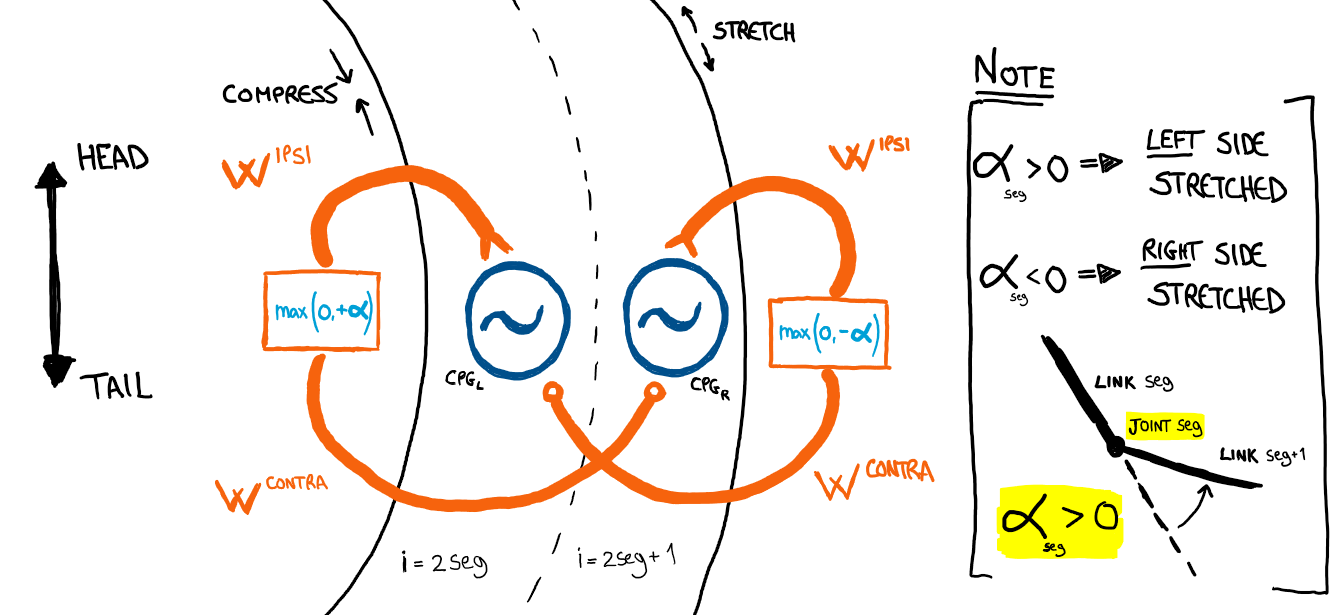
\includegraphics[width=\textwidth]{figures/CPG_scheme.png}}
  \end{subfigure}
  \caption{\label{fig:cpg_scheme} Schematics of the proprioceptive sensory feedback}
\end{figure}


The local proprioceptive feedback $s_i$ for oscillator $i$ is calculated as the sum of the effect
from ipsilateral and contralateral feedback, paying attention to the considered side.

For the LEFT oscillator at segment/joint $seg$ ($i = 2seg$):
\begin{equation}
  \label{eq:stot_left}
 s_i = W^{ipsi}max(0, +\alpha_{seg}) + W^{contra}max(0, -\alpha_{seg})
\end{equation}

For the RIGHT oscillator at segment/joint $seg$ ($i = 2seg + 1$):
\begin{equation}
  \label{eq:stot_right}
  s_i = W^{ipsi}max(0, -\alpha_{seg}) + W^{contra}max(0, +\alpha_{seg})
\end{equation}

Note that the feedback signal is only computed from the stretched side of the body, while
compression part is not considered.
For ease of implementation, we provide a reference feedback weight value $ws\_ref$,
computed as the inverse of the average joint angles that you used also for Project 1.
The value of $ws\_ref$ is provided in \fileref{util/zebrafish\_hyperparameters.py}.
In your code, you will modulate the reference value by two parameters
for the ipsilateral ($w_{ipsi}$) and contralateral ($w_{contra}$) components, according to

 \begin{eqnarray}
  \label{eq:s_weight}
  W^{ipsi}   = ws\_ref * w_{ipsi}    \quad \\
  W^{contra} = ws\_ref * w_{contra}
\end{eqnarray}

After including proprioceptive feedback, the oscillator equations have to be updated:


\begin{equation}
  \label{eq:damplitude}
  \dot{r}_i = a(R_i-r_i)+s_icos(\theta_i)
\end{equation}

with $ r_i $ the
oscillator amplitude, $ R_i $ the nominal amplitude, $\theta_i$ the oscillator phase.

\begin{equation}
  \label{eq:dphase}
  \dot{\theta}_i = 2 \pi f + \sum_j r_j w_{ij} sin(\theta_j - \theta_i - \phi_{ij}) - \frac{s_i}{R_i}sin(\theta)
\end{equation}

with $ f $ the frequency, $ r_i $ the
oscillator amplitude, $ w_ij $ the coupling weights, $\theta_i$ the oscillator phase.

\textbf{Correction of project 1: }
Note that in Project 1 Eqn.4 and Eqn.5, we only implemented the coupling from left to right side,
which worked in open-loop. For a closed-loop CPG, we need the coupling to be mutual:

\begin{equation}
  \label{eq:dcw}
  w_{ij} =
    \begin{cases}
    w_{body2body},& \text{if } |i-j|=2 \\
    w_{body2body\_contralateral}, & \text{if }  j-i=1 \text{ and } i\%2=0\\
    w_{body2body\_contralateral}, & \text{if }  i-j=1 \text{ and } i\%2=1 \text{ \textbf{(mutual)} }\\
    0, & \text{otherwise} \\
    \end{cases}
\end{equation}

\begin{equation}
  \label{eq:phicw}
  \phi_{ij} =
    \begin{cases}
    sign(i-j)\cdot\frac{\phi_{body\_total}}{n_{joints}-1},& \text{if } |i-j|=2 \\
    sign(i-j)\cdot\pi,&  \text{if }  j-i=1 \text{ and } i\%2=0\\
    sign(i-j)\cdot\pi,& \text{if }   i-j=1 \text{ and } i\%2=1 \text{ \textbf{(mutual)} }\\
    0, & \text{otherwise} \\
    \end{cases}
\end{equation}

\textbf{\underline{Question 5.1} Update \fileref{abstract\_oscillator\_controller.py} to implement the stretch feedback.}

\textbf{\underline{Question 5.2} Test your implementation by running the network using \fileref{exercise5.py} with default values $W^{ipsi}=0.25 * ws_{ref}$ and $W^{contra}=-0.25 * ws_{ref}$. Plot the oscillator phases evolution, oscillator amplitudes evolution, motor output and motor output difference evolution, and the zebrafish joint angles evolution vs time. Observe the result and analyze how it changes compared to open-loop CPGs}

\textbf{\underline{Question 5.3} Report the controller and mechanical metrics of the simulation.  Record a video of the zebrafish swimming for 10s}.

\textbf{\underline{Question 5.4} Test different feedback weight values for ipsilateral and contralateral feedback connections in \fileref{exercise6.py}. Keep $w^{ipsi}=0$ and test $w^{contra}$ in range [-1,1] scaled by $ws\_ref$. Keep $w^{contra}=0$ and test $w^{ipsi}$ in range [-1,1] scaled by $ws\_ref$. $ws\_ref$ is the inverse of average joint amplitudes (provided in the code). Plot the neural controller (neural frequency, total wave lag ) and mechanical metrics (cost of transport, energy consumption, forward speed, joint amplitudes, sum of torques) as a function of different ipsilateral and contralateral feedback strengths.}.

\textbf{\underline{Question 5.5} Analyze the result qualitatively in Describe the effect of ipsilateral and contralateral feedbacks on the swimming locomotion behaviors. How does it relate from the observation (at the beginning of the section) about the known sensory neurons?}.

\subsection*{6. Swimming under perturbations}

In the lamprey it has been shown that an external rhythmic bending, imposed during the activation of the CPG network, has the capability to modulate the frequency of the ongoing oscillations so that they synchronize with the external stimulus. This synchronization is made possible by the proprioceptive sensory neurons and their direct connections to the CPG segments.

In this exercise, we test the stability of the closed-loop CPG controller under external perturbations. Specifically, we apply a rhythmic bending (entrainment) of 45 degrees with a fixed frequency on the axial joints. The implementation of the rhythmic bending is already provided in a helper function \fileref{define\_entraining\_signals} (check \fileref{util/entraining\_signals.py} for detailed implementations and you need to pass the output of entraining\_signals in the SimulationParameters class to access the prescribed kinematics given by entraining\_signals in network\_ode).

Hint: Since we're imposing a movement on the zebrafish, the joint positions are already known and we don't need to do a full physical simulation.
If you still want to visualize the swimming behavior, import \fileref{run\_single} from \fileref{util.run\_closed\_loop} instead of \fileref{util.run\_open\_loop}.

\textbf{\underline{Question 6.1} Explore the entrainment by running \fileref{exercise7.py}, where a default entrainment of 45 degrees at 8 Hz is implemented. Report the neural frequency of the controller. How does the frequency compare to the simulation without entrainment? Does this match your expectation and why?}

\textbf{\underline{Question 6.2} Explore the effect of the entrainment on the neural frequency under different feedback gain strengths systematically in \fileref{exercise8.py}. For simplicity, we take $w^{ipsi} = -w^{contra} = w$
Specifically, run the simulation with feedback gains $w$ in range [0,2] scaled by $ws\_ref$ and entrainment frequencies in range [3.5,10] in a 2D grid. Take $w=0$ (no feedback) as a reference baseline with reference neural frequency. Plot the difference between the entrainment frequency and the reference frequency vs. the difference between the actual resulting neural frequency and the reference frequency. Describe and qualitatively analyze your observations.}



\subsection*{7. CPG-free swimming with proprioceptive feedback}

In last parts of the project we implemented an open-loop CPG and a closed-loop CPG with sensory feedback. Now we want to study if the local proprioceptive feedback alone is enough to elicit the swimming behavior.

\textbf{\underline{Question 7.1} Try removing the ipsilateral connection from the CPG model while preserving the stretch feedback in \fileref{exercise9.py}. Test if the fish could still initiate the swimming behavior. Does the result change if you alter the feedback strengths? Summarize and explain your observations and use plots/videos if needed.}

\textbf{\underline{Question 7.2} Repeat the experiments and try removing the contralateral connections or both ipsilateral and contralateral connections. Can you still generate the swimming behavior? If yes, report the feedback parameters used, record a video, and analyze how the CPG-free swimming compares to CPG swimming. If not, analyze the minimum CPG connections needed to elicit a swimming behavior.
}



%% -----------------------------SOLUTION ------------------------------


\bibliographystyle{ieeetr}
\bibliography{cmc_2025}
\label{sec:references}





% \newpage

% \section*{APPENDIX}
% \label{sec:appendix}

\end{document}

%%% Local Variables:
%%% mode: latex
%%% TeX-master: t
%%% End: